\textit{Response.}

\begin{enumerate}[a)]
	\item Source code is available from the GitHub repository
	
	\begin{center}
		\url{https://github.com/jasonltorchinsky/MATH833_HW/releases/tag/hw4}
	\end{center}

	and is given in Appendix~\ref{app:code_3a}. In short, the code takes a input parameters \texttt{-a}, \texttt{-f}, and \texttt{-s}, which correspond to $a$, $f$, and $\sigma$, respectively. The code then simulates 250 individual realizations of the linear stochastic differential equation (SDE) with multiplicative noise using the Euler--Maruyama method with time-step size $\Delta t = 0.01$, and generates the plots included below
	
	\begin{figure}[H]
		\centering
		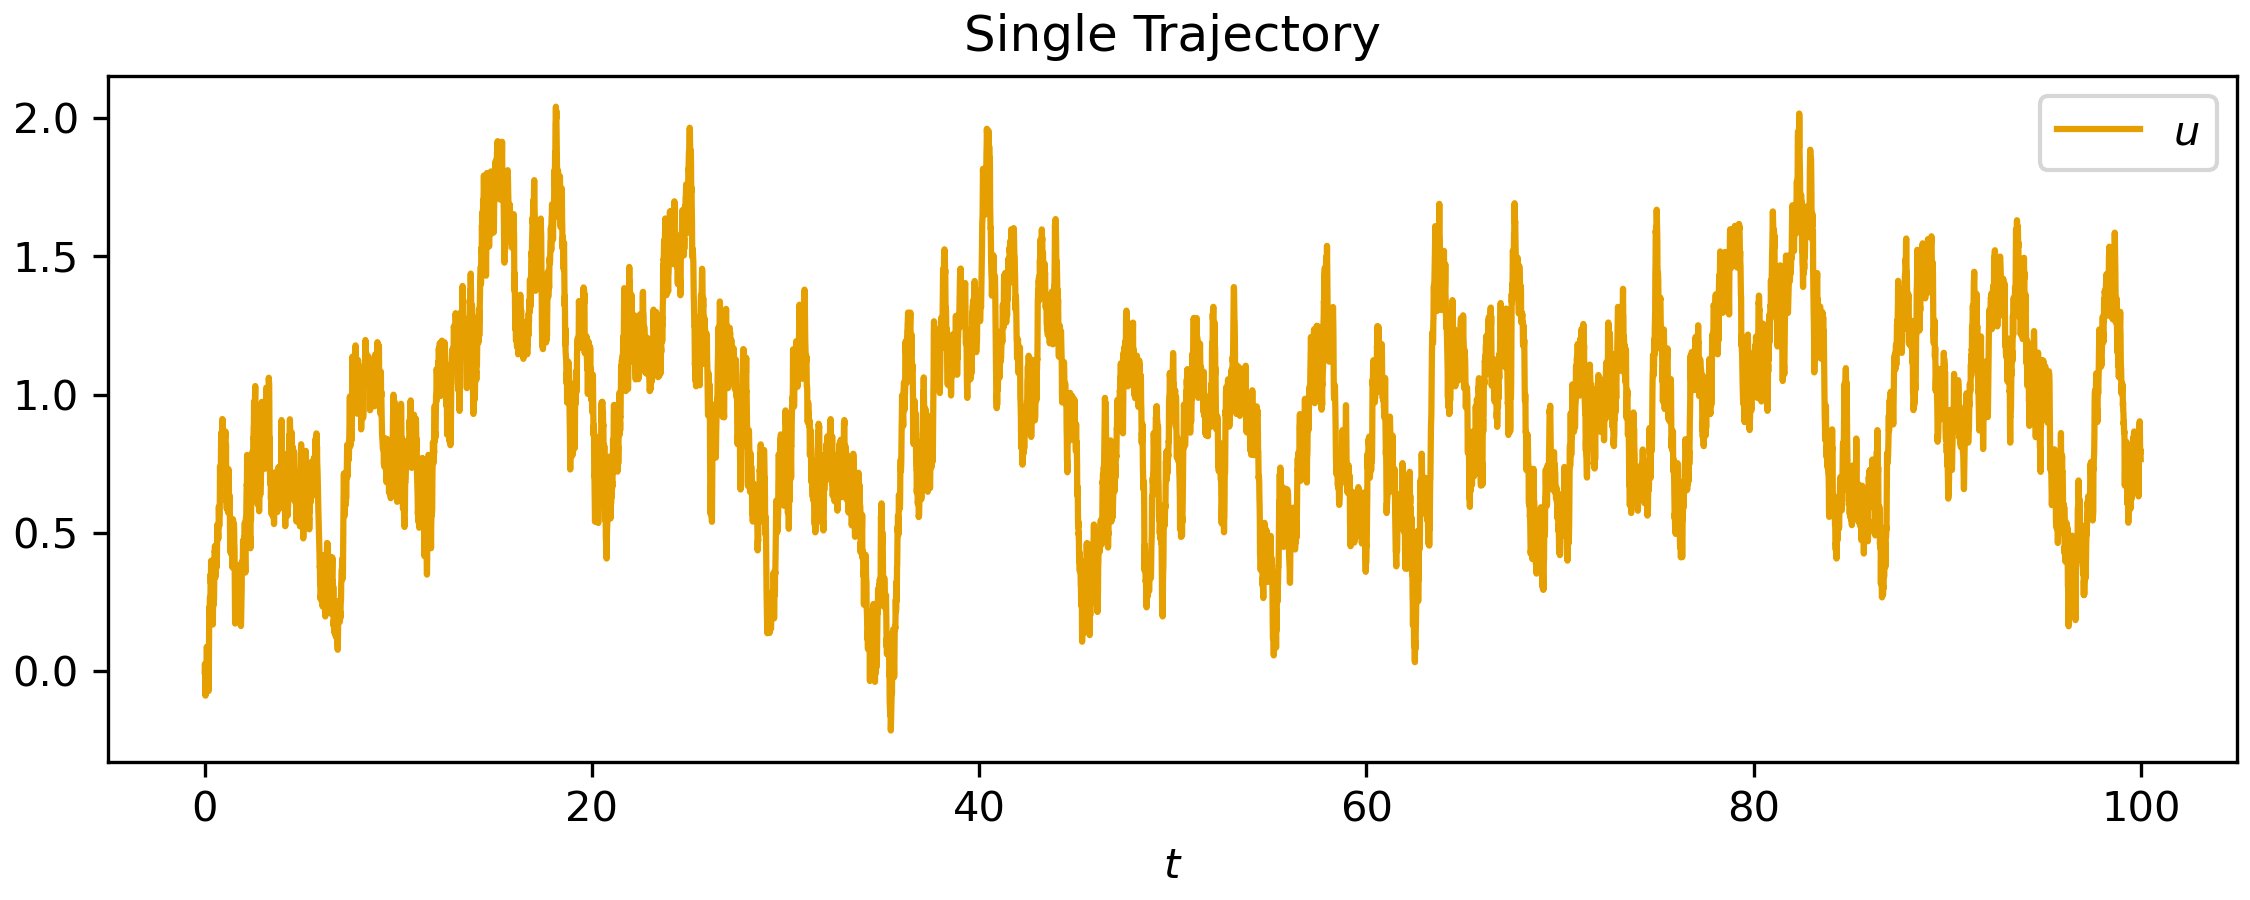
\includegraphics[width=0.75\textwidth]{../../src/3a_traj.png}
		\caption{A single realization of the SDE with parameters $a = f = 1$ and $\sigma = 0.5$ with initial condition $u = 0$ and time-step size $\Delta t = 0.01$. }
		\label{fig:3a_traj}
	\end{figure}
	
	\begin{figure}[H]
		\centering
		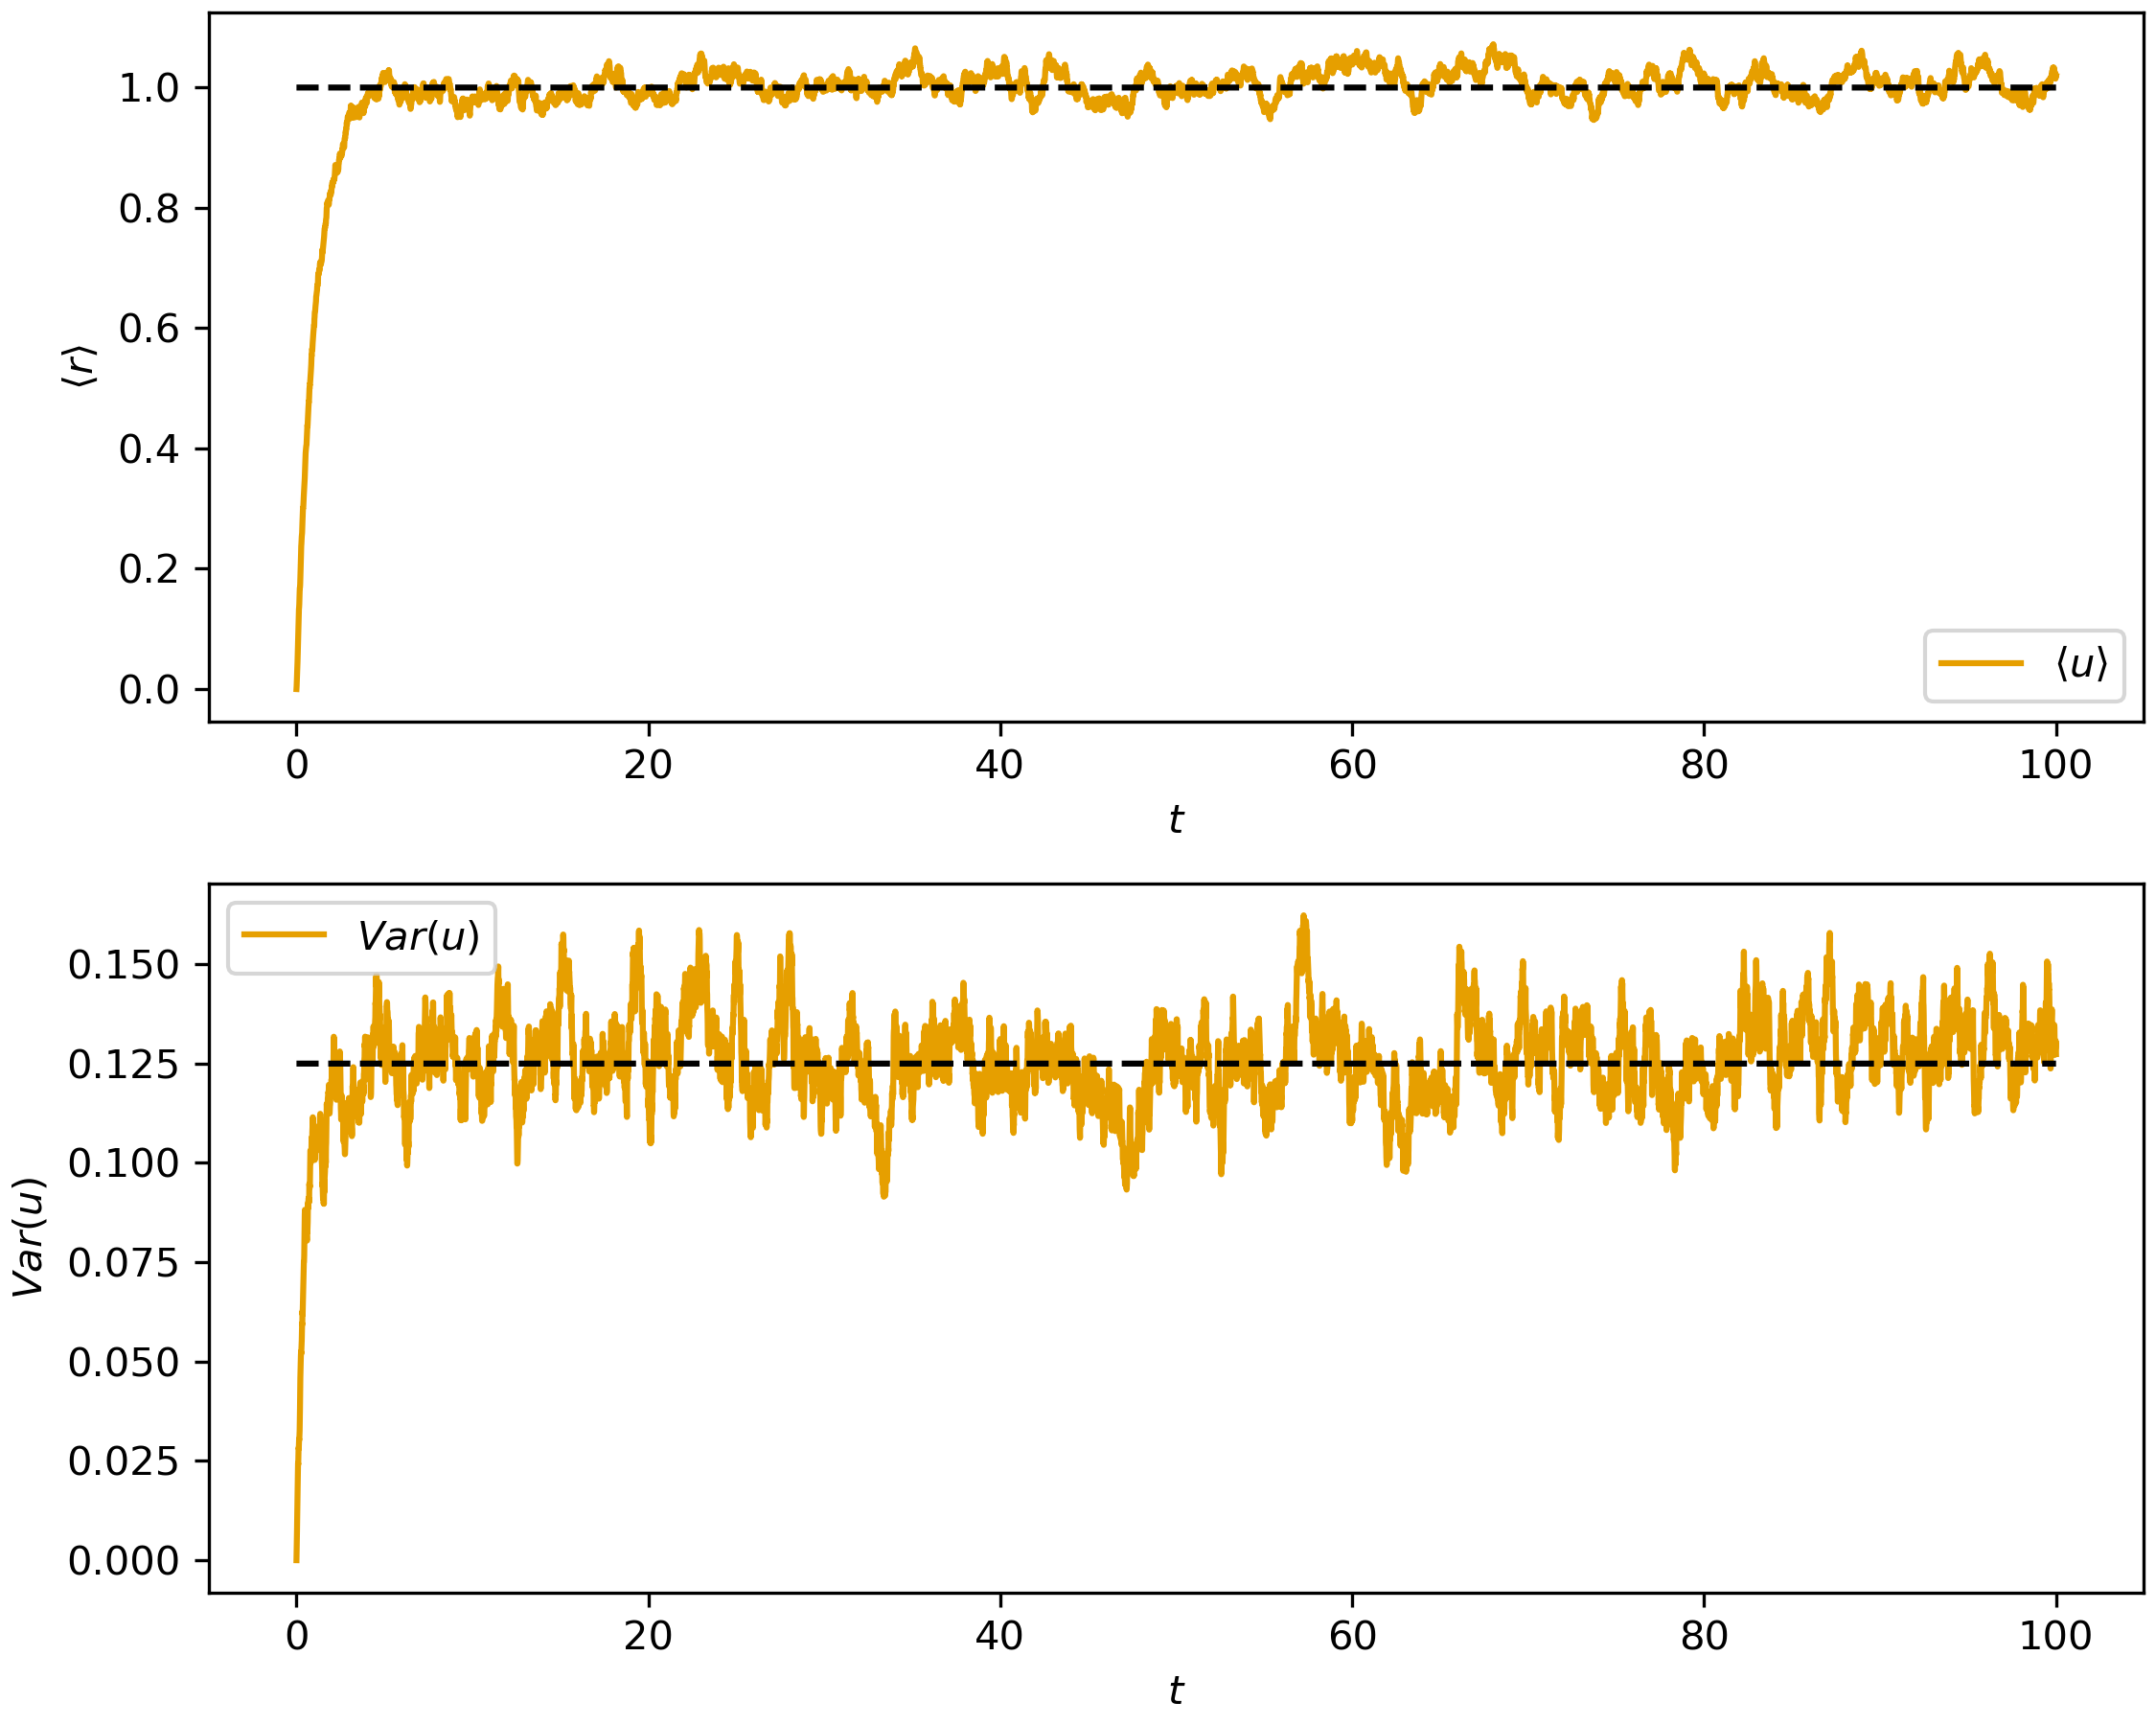
\includegraphics[width=0.75\textwidth]{../../src/3a_ens_stats.png}
		\caption{The evolution of ensemble mean (top) and variance (bottom) of the SDE with parameters $a = f = 1$ and $\sigma = 0.5$ across 250 trials, with initial condition $u = 0$ and time-step size $\Delta t = 0.01$ for all trials. }
		\label{fig:3a_ens_stats}
	\end{figure}
	
\end{enumerate}

